\documentclass[10pt,a4paper]{article}
\usepackage[utf8]{inputenc}
\usepackage[francais]{babel}
\usepackage[T1]{fontenc}
\usepackage{amsmath}
\usepackage{amsfonts}
\usepackage{amssymb}
\usepackage{graphicx}
\usepackage{amsthm}
\usepackage{systeme}
\usepackage{stmaryrd}

\theoremstyle{definition}
\newtheorem{definition}{Définition}
\theoremstyle{theorem}
\newtheorem{theorem}{Théorème}

\author{Della Bona Sarah, Dumez Erika}
\title{Introduction to neural ODE}
\begin{document}
\maketitle
 
 
\section{Ordinary Differential Equations}

\subsection{A refresher on ODE}

An ODE is a function that describes the changes of a function, $u$, through time. In this setting, time is a continuous variable and we don't know the real function, only its derivative.

\begin{definition}
Let $f: \Omega \subseteq \mathbb{R} x \mathbb{R}^N \rightarrow \mathbb{R}^N$. 

A \textit{first order ODE} takes of the form:
\[
\partial_t u(t) = f(t,u(t)) \textbf{   (1)}
\]

\begin{itemize}
\item A \textit{solution} for (1) is a function $u : I \rightarrow \mathbb{R}^N$ where $I$ is an interval of $\mathbb{R}$ such that:
	\begin{itemize}
	\item u is derivable on I,
	\item $\forall t \in I, f(t, u(t)) \in \Omega$,
	\item $\forall t \in I, \partial_t u(t) = f(t, u(t))$
	\end{itemize}
\item An \textit{initial condition} (IC) is a condition of the type:
\[
u(t_0) = u_0
\]
where $(t_0, u_0) \in \Omega$ is fixed.
\end{itemize}
\item A \textit{Cauchy problem} is an ODE with IC
\[
\left \{
\begin{array}{rcl}
\partial_t u(t) & = & f(t, u(t)) \\
u(t_0) & = & u_0
\end{array}
\right.
\]
\end{definition}

\begin{definition}
A \textit{k-order ODE} is of the form:
\[
\partial^k_t v(t) = g(t, v(t), ... , \partial^{k-1}v(t))
\]
where 
   \begin{eqnarray}
   \nonumber
   v & : & I \rightarrow \mathbb{R}^N \\ 
   \nonumber
   g & : & \Theta \subseteq \mathbb{R} \times \mathbb{R}^N \times ... \times \mathbb{R}^N \rightarrow \mathbb{R}^N
   \end{eqnarray}
\end{definition}

It is not always possible to explicitly find a solution to a Cauchy problem, but we can compute a finite number of points $u_i \in \mathbb{R}^N$ which are close to the real solution. 

More precisely, let $T \in \mathbb{R}\\\{0\}$ such that the solution $u$ exists on $[t_0, t_0 + T]$ and let $n \in \mathbb{N}^{\geqslant 2}$. We are then looking for $(u_i)^n_{i=0}$ s.t. 
\[
u_i \approx u(t_i) \ \text{ where } t_0 < ... < t_n \in [t_0, t_0 + T]
\]

Let $h_i := t_{i+1} - t_i$, it is called the \textit{step}. To compute those $u_i$, we use \textit{1-step methods} such as Euler's method.

\subsection{Euler's method}

Euler's method is similar to a Taylor development, the idea is to compute $u(t_{i+1})$ using the following formula:\footnote{We consider that $ \forall i\ \{0,...,n\}, h_i = h$.}
\[
u(t_{i+1}) \approx u(t_i) + h . \partial u(t_i)
\]
where 
\[
\partial u(t_i) = f(t_i, u(t_i)).
\]

\section{Neural networks}

In a typical machine learning problem, you are given some input $x$ and you want to predict an output $y$. A \textit{neural network} can be used to solve such a problem. It consists of a series of layers. These layers are matrix operations. The first layer takes an input and the result of the computation on that input is given to the hidden layers. An hidden layer takes an input from the previous layer and compute an output for the next. The last layer returns the final output, the prediction. 

We can see a neural network as a composite of functions, a function for each layer. That is because each layer uses an activation function on its input. 

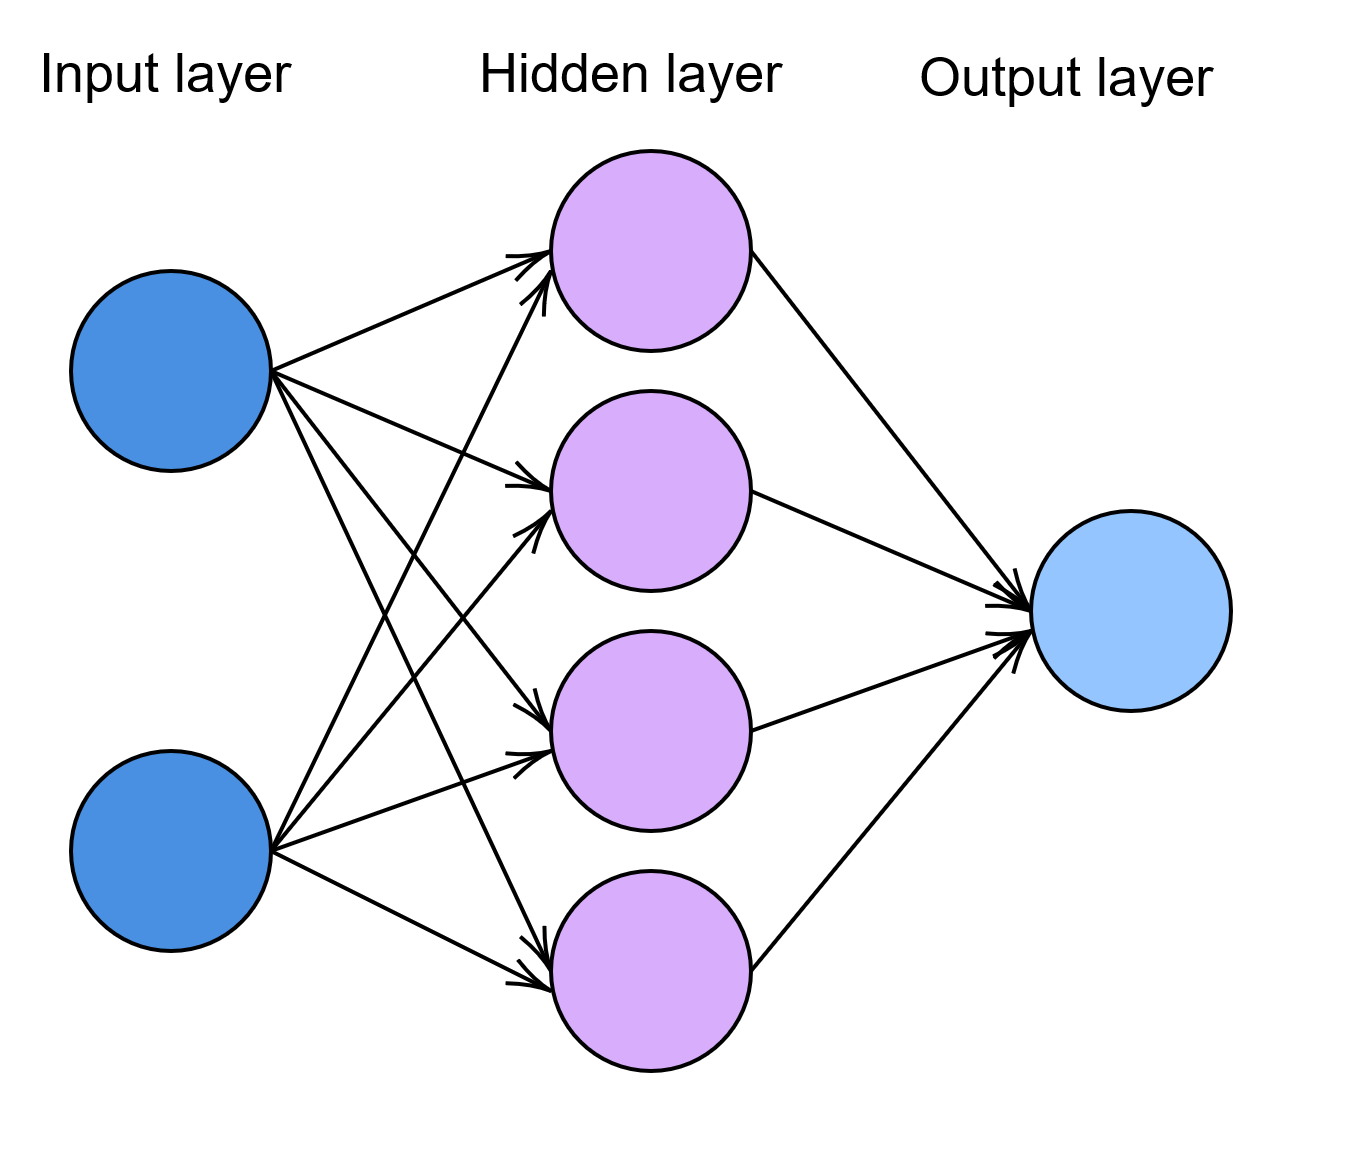
\includegraphics[scale=0.7]{nn.png}

Each layer introduces a little bit of error that propagate through the network. 

\subsection{Example}

Let's consider a neural network, with one hidden layer, that takes a 2-dimensional input $x = (x_1, x_2)$, and gives a 2-dimensional output $y = (y_1,y_2)$. We can represent this network with the following equations:

   \begin{eqnarray}
   \nonumber
   z_i & = & \sum_{j=1}^2 w_{ij}^{(1)}x_j + b_i^{(1)} \text{ pour } i = 1,2 \\ 
   \nonumber
   h_i & = & \sigma (z_i) \text{ pour } i=1,2 \\
   \nonumber
   y_k & = & \sum_{i=1}^2 w_{ki}^{(2)}h_i + b_k^{(2)} \text{ pour } k = 1,2 \\
   \nonumber
   \mathcal{L} & = & \frac{1}{2} \sum_{k = 1}^2 (y_k - t_k)^2
   \end{eqnarray}
   
where $w^{(1)}$, $w^{(2)}$, $b^{(1)}$ and $b^{(2)}$ are parameters of the network, and $t = (t_1, t_2)$ is the value we want to approximate (the "real" output for $x$). 

\subsection{Back propagation}

\section{Residual neural network theory}

Residual networks have the best accuracy. The only change to a regular neural network is that we not only feed the output of the previous layer to the next, but also the input of that layer. It creates skip connections, so that the network can decide how deep it needs to be. As a formula, the $k+1$th layer has the formula:
\[
x_{k+1} = x_k + F(x_k)
\]
where $F$ is the function of the $k$th layer and its activation. This simple formula is a special case of the formula:
\[
x_{k+1} = x_k + h.F(x_k),
\]
which is the formula for the Euler method for solving ordinary differential equations (ODEs) when $h = 1$. It is with this observation that we can introduce neural ODE.


\section{Neural ODE}

\subsection{Introduction}

(In this case, the initial condition for the system is "time" $0$, which indicates the very first layer of the neural network, and as $x(0)$ will serve the normal input. The final condition at "time" $t$ will be the desired output of the neural network: a scalar value, a vector representing classes or anything else.
These residuals connections are discretised time steps of the Euler method, it means that we can regulate the depth of the neural network, just with choosing the discretising scheme, hence, making the solution (aka the neural network) more or less accurate, even making it infinite-layer like. )

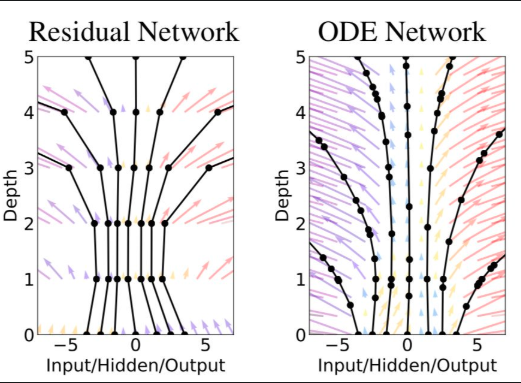
\includegraphics[scale=1]{resnetvsodenet.png}



\subsection{definition?}

\subsection{Forward pass}

\subsection{Adjoint method}
 
\subsection{Backwward pass}

\subsection{Advantages and disadvantages  }

In regular neural networks, we consider discrete, individual and independent layers. They are just a block of operations and the neural network consists of those blocks. However, ODE network can be seen as continuous functions. Instead of having separate layers, the entire network is one continuous block of computation. This leads to many advantages but also some disadvantage:
\begin{itemize}
\item The most benefit is that ODENet has more accurate results for time series predictions. Regular neural network have discrete layers, which means they expect the intervals for these time series data sets to be fixed. Therefore, they are bad at predicting output for time series data that is irregular.
\item They have a faster testing time than regular networks, but a slower training time. Thus it's perfect for low power edge computing. There is a trade-off between precision and speed.
\item We can use ordinary differential equations solvers instead of gradient descent. These solvers have a hundred plus years of theory behind them.
\item Lastly, there's a constant memory cost, instead of increasing the cost linearly with each layer in a regular network.
\end{itemize}








\textbf{voir def vector field}

\textbf{voir probleme du vanishing gradient dans les nn regulier}

\textbf{ recherche the Universal Approximation Theorem states that, for enough layers or enough parameters, $ML(x)$ can approximate any nonlinear function sufficiently close (subject to some constraints).}







% https://julialang.org/blog/2019/01/fluxdiffeq/

This generation of a prediction $y$ from $x$ is a machine learning model ($ML$). During training, we attempt to adjust the parameters of $ML$ so that it generates accurate predictions. $y = ML(x)$. The reason $ML$ is interesting is because its form is basic but adapts to the data itself. The theory and practice of machine learning confirms that this is a good way to learn nonlinearities.  For example, 



Instead of learning the nonlinear transformation directly, we wish to learn the structures of the nonlinear transformation. Thus, instead of doing $y = ML(x)$, we put the machine learning model on the derivative, $y'(x) = ML(x)$, and now we solve the ODE. Why do this? One motivation is that defining the model in this way and then solving the ODE using the simplest and most error prone method, the Euler method, what we get is equivalent to a residual neural network. Rather than adding more layers, we can just model the differential equation directly and then solve it using a purpose-built ODE solver. 

\textbf{Let's put an ODE into a neural net framework!}

To understand embedding an ODE into a neural network, let's look at what a neural network layer actually is. A layer is really just a differentiable function which takes in a vector of size $n$ and spits out a new vector of size $m$. 
Turns out that differential equations solvers fit this framework, too: a solve takes in some vector $p$ (which might include parameters like the initial starting point), and outputs some new vectors, the solution. Moreover it's differentiable, which means we can put it straight into a larger differentiable program. This larger program can happily include neural networks, and we can keep using standard optimisation techniques like ADAM to optimise their weights.

% https://stats.stackexchange.com/questions/445562/what-are-the-practical-uses-of-neural-odes

For time series and density modelling, neural ODEs offer some benefits that we don't know how to get otherwise. For plain supervised learning, there are potential computational benefits, but for practical purposes they probably aren't worth using yet in that setting.

Neural ODEs differ in two ways from standard nets:

\begin{enumerate}
\item They represent a different set of functions, which can be good or bad depending on what you're modelling.
\item We have to approximate their exact solution, which gives more freedom in how to compute the answer, but adds complexity.
\end{enumerate}

The clearest setting where neural ODEs help is building continuous-time series models, which can easily handle data coming at irregular intervals. However, ODEs can only model deterministic dynamics. 

Conventional nets can be evaluated exactly with a fixed amount of computation, and are typically faster to train. Plus, with standard nets you don't have to choose an error tolerance for a solver.











(Here, let's consider a neural network as a continuous function with no grouping, no blocks. Instead of having single layers, we have the entire network be one continuous block of computation. This means that we do not need to specify the number of layers beforehand. We normally have to decide how many layers we want in our neural network, and then we can build the network. With this idea, instead of specifying the number of layers, we need to specify the desired accuracy of the function, and it will learn how to train itself within that margin of error. )





























\end{document}